\documentclass{standalone}
\usepackage{tikz}
\usetikzlibrary{patterns, positioning}
\usepackage[sfdefault]{ClearSans} %% option 'sfdefault' activates Clear Sans as the default text font
\usepackage[T1]{fontenc}

\begin{document}
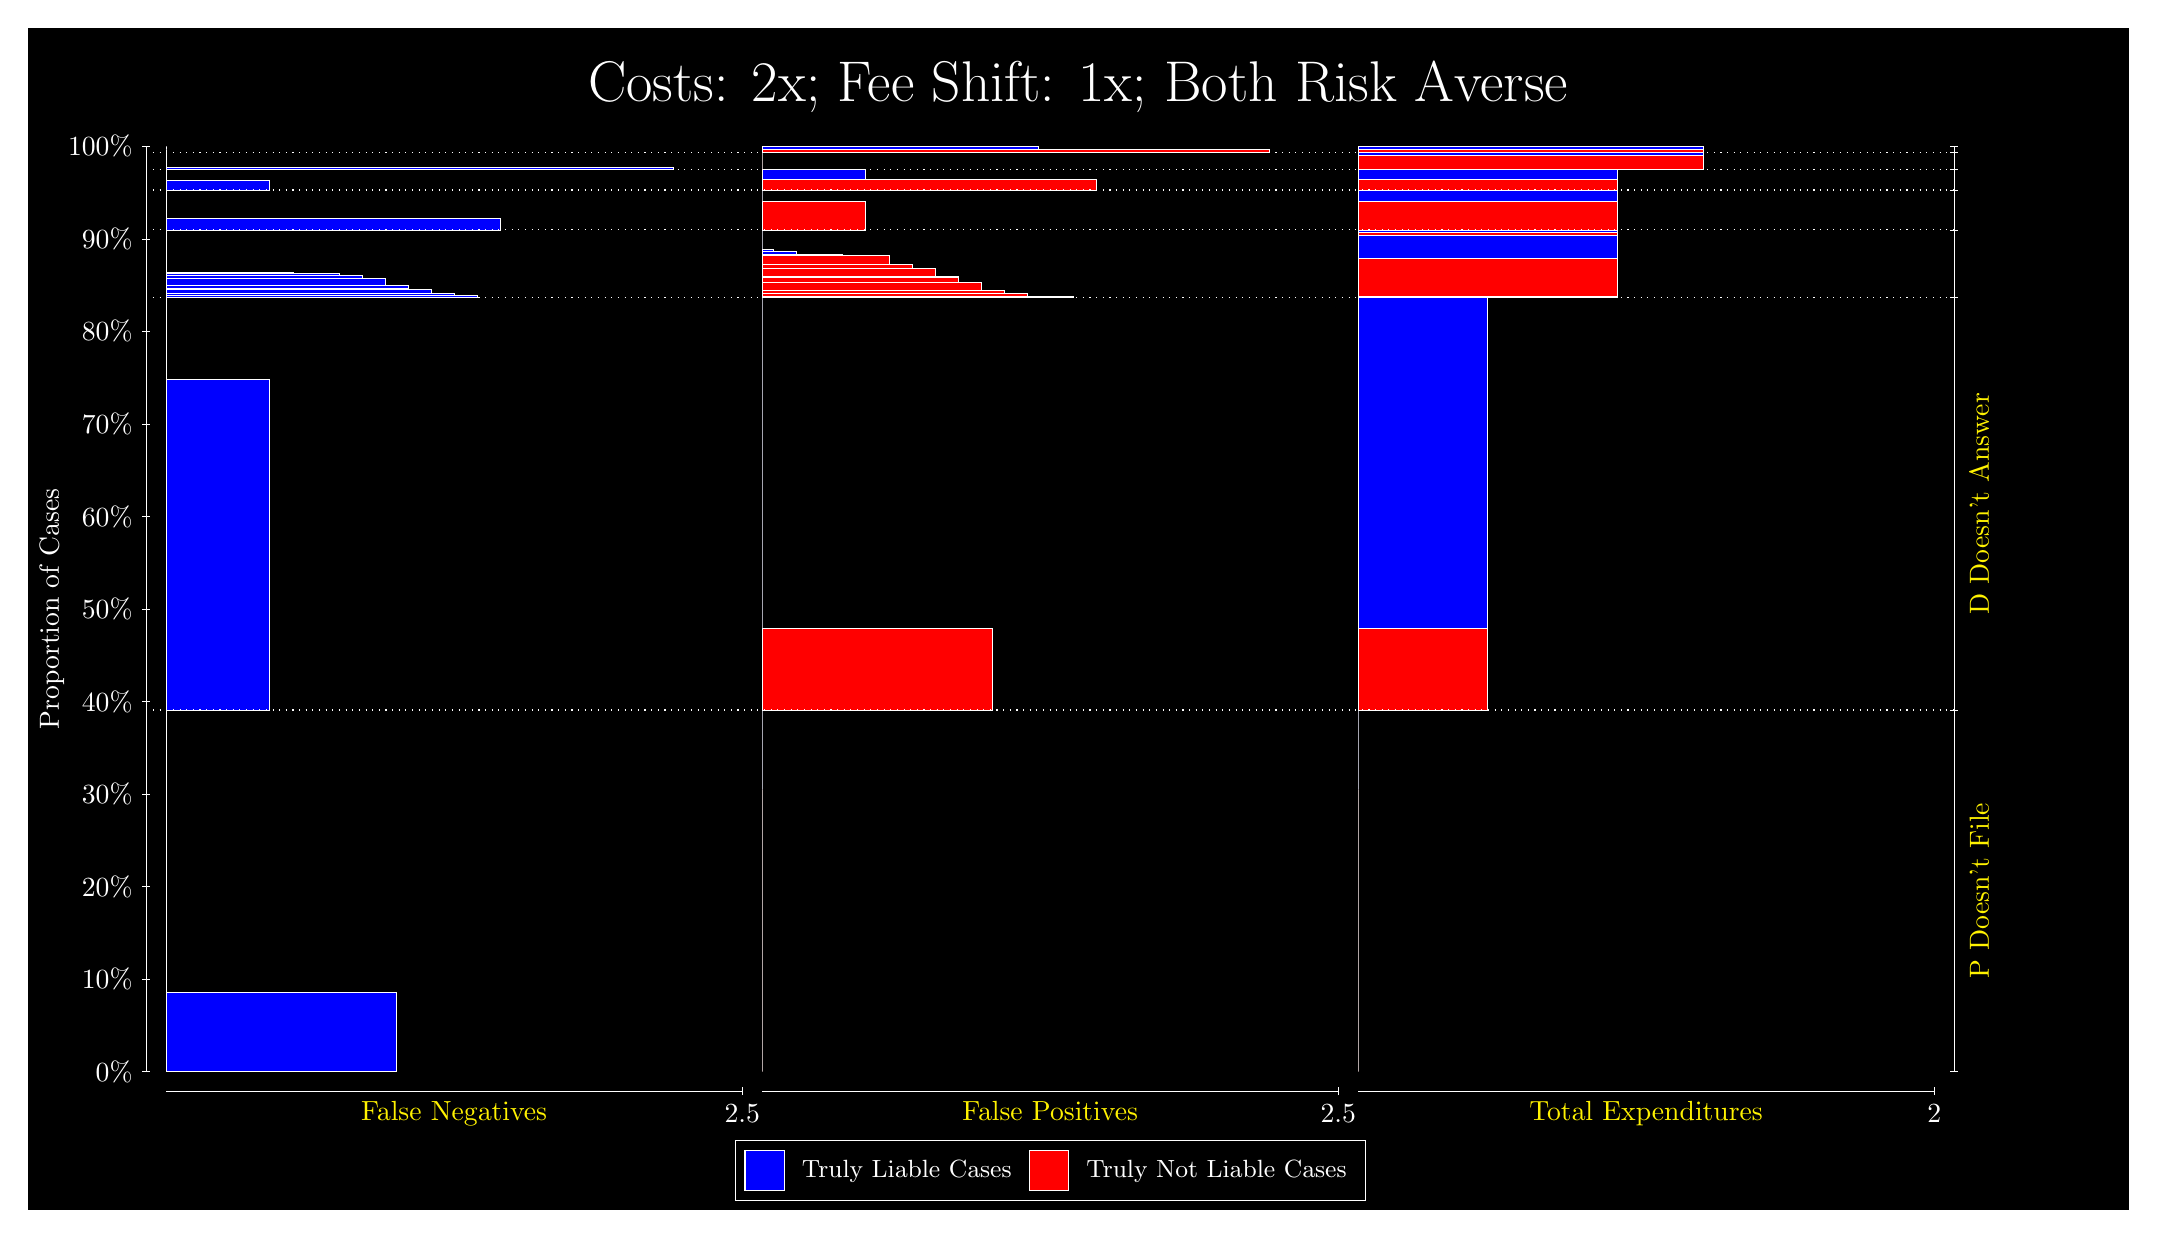
\begin{tikzpicture}
\draw[fill=black] (0,0) rectangle (26.667,15);
\draw[text=white] (0,13.5) rectangle (26.667,15) node[midway] {\huge Costs: 2x; Fee Shift: 1x; Both Risk Averse};
\draw[white, very thin] (1.5,1.75) -- (1.5,13.5);
\node[rotate=90, text=white, anchor=center] at (0.3, 7.625) {Proportion of Cases};
\draw[white, very thin] (1.45,1.75) -- (1.55,1.75);
\node[text=white, anchor=east] at (1.45, 1.75) {0\%};
\draw[white, very thin] (1.45,2.925) -- (1.55,2.925);
\node[text=white, anchor=east] at (1.45, 2.925) {10\%};
\draw[white, very thin] (1.45,4.1) -- (1.55,4.1);
\node[text=white, anchor=east] at (1.45, 4.1) {20\%};
\draw[white, very thin] (1.45,5.275) -- (1.55,5.275);
\node[text=white, anchor=east] at (1.45, 5.275) {30\%};
\draw[white, very thin] (1.45,6.45) -- (1.55,6.45);
\node[text=white, anchor=east] at (1.45, 6.45) {40\%};
\draw[white, very thin] (1.45,7.625) -- (1.55,7.625);
\node[text=white, anchor=east] at (1.45, 7.625) {50\%};
\draw[white, very thin] (1.45,8.8) -- (1.55,8.8);
\node[text=white, anchor=east] at (1.45, 8.8) {60\%};
\draw[white, very thin] (1.45,9.975) -- (1.55,9.975);
\node[text=white, anchor=east] at (1.45, 9.975) {70\%};
\draw[white, very thin] (1.45,11.15) -- (1.55,11.15);
\node[text=white, anchor=east] at (1.45, 11.15) {80\%};
\draw[white, very thin] (1.45,12.325) -- (1.55,12.325);
\node[text=white, anchor=east] at (1.45, 12.325) {90\%};
\draw[white, very thin] (1.45,13.5) -- (1.55,13.5);
\node[text=white, anchor=east] at (1.45, 13.5) {100\%};

\draw[white, very thin] (24.457,1.75) -- (24.457,13.5);
\draw[white, very thin] (24.407,1.75) -- (24.507,1.75);
\node[anchor=west] at (24.407, 1.75) {};
\draw[white, very thin] (24.407,6.342) -- (24.507,6.342);
\node[anchor=west] at (24.407, 6.342) {};
\draw[white, very thin] (24.407,11.579) -- (24.507,11.579);
\node[anchor=west] at (24.407, 11.579) {};
\draw[white, very thin] (24.407,12.44) -- (24.507,12.44);
\node[anchor=west] at (24.407, 12.44) {};
\draw[white, very thin] (24.407,12.945) -- (24.507,12.945);
\node[anchor=west] at (24.407, 12.945) {};
\draw[white, very thin] (24.407,13.204) -- (24.507,13.204);
\node[anchor=west] at (24.407, 13.204) {};
\draw[white, very thin] (24.407,13.424) -- (24.507,13.424);
\node[anchor=west] at (24.407, 13.424) {};
\draw[white, very thin] (24.407,13.5) -- (24.507,13.5);
\node[anchor=west] at (24.407, 13.5) {};

\draw[white, very thin, fill=blue] (1.75,1.75) rectangle (4.6775,2.759);
\draw[white, very thin, fill=red] (1.75,2.759) rectangle (1.75,6.342);
\draw[white, very thin, fill=blue] (1.75,6.342) rectangle (3.0674,10.539);
\draw[white, very thin, fill=red] (1.75,10.539) rectangle (1.75,11.579);
\draw[white, very thin, fill=blue] (1.75,11.579) rectangle (5.7022,11.612);
\draw[white, very thin, fill=blue] (1.75,11.612) rectangle (5.4094,11.63);
\draw[white, very thin, fill=blue] (1.75,11.63) rectangle (5.1167,11.684);
\draw[white, very thin, fill=blue] (1.75,11.684) rectangle (4.8239,11.692);
\draw[white, very thin, fill=blue] (1.75,11.692) rectangle (4.8239,11.738);
\draw[white, very thin, fill=blue] (1.75,11.738) rectangle (4.5312,11.826);
\draw[white, very thin, fill=blue] (1.75,11.826) rectangle (4.2384,11.858);
\draw[white, very thin, fill=blue] (1.75,11.858) rectangle (3.9457,11.886);
\draw[white, very thin, fill=blue] (1.75,11.886) rectangle (3.6529,11.894);
\draw[white, very thin, fill=blue] (1.75,11.894) rectangle (3.3602,11.903);
\draw[white, very thin, fill=red] (1.75,11.903) rectangle (1.75,12.44);
\draw[white, very thin, fill=blue] (1.75,12.44) rectangle (5.9949,12.59);
\draw[white, very thin, fill=red] (1.75,12.59) rectangle (1.75,12.945);
\draw[white, very thin, fill=blue] (1.75,12.945) rectangle (3.0674,13.064);
\draw[white, very thin, fill=red] (1.75,13.064) rectangle (1.75,13.204);
\draw[white, very thin, fill=blue] (1.75,13.204) rectangle (8.1906,13.238);
\draw[white, very thin, fill=red] (1.75,13.238) rectangle (1.75,13.424);
\draw[white, very thin, fill=red] (1.75,13.424) rectangle (1.75,13.458);
\draw[white, very thin, fill=blue] (1.75,13.458) rectangle (1.75,13.5);
\draw[white, very thin, fill=red] (9.3189,1.75) rectangle (9.3189,5.333);
\draw[white, very thin, fill=blue] (9.3189,5.333) rectangle (9.3189,6.342);
\draw[white, very thin, fill=red] (9.3189,6.342) rectangle (12.246,7.3824);
\draw[white, very thin, fill=blue] (9.3189,7.3824) rectangle (9.3189,11.579);
\draw[white, very thin, fill=red] (9.3189,11.579) rectangle (13.271,11.59);
\draw[white, very thin, fill=red] (9.3189,11.59) rectangle (12.978,11.601);
\draw[white, very thin, fill=red] (9.3189,11.601) rectangle (12.686,11.635);
\draw[white, very thin, fill=red] (9.3189,11.635) rectangle (12.393,11.678);
\draw[white, very thin, fill=red] (9.3189,11.678) rectangle (12.1,11.775);
\draw[white, very thin, fill=red] (9.3189,11.775) rectangle (11.807,11.833);
\draw[white, very thin, fill=red] (9.3189,11.833) rectangle (11.807,11.847);
\draw[white, very thin, fill=red] (9.3189,11.847) rectangle (11.515,11.952);
\draw[white, very thin, fill=red] (9.3189,11.952) rectangle (11.222,11.998);
\draw[white, very thin, fill=red] (9.3189,11.998) rectangle (10.929,12.116);
\draw[white, very thin, fill=blue] (9.3189,12.116) rectangle (10.344,12.125);
\draw[white, very thin, fill=blue] (9.3189,12.125) rectangle (10.051,12.134);
\draw[white, very thin, fill=blue] (9.3189,12.134) rectangle (9.758,12.161);
\draw[white, very thin, fill=blue] (9.3189,12.161) rectangle (9.4652,12.193);
\draw[white, very thin, fill=blue] (9.3189,12.193) rectangle (9.3189,12.44);
\draw[white, very thin, fill=red] (9.3189,12.44) rectangle (10.636,12.796);
\draw[white, very thin, fill=blue] (9.3189,12.796) rectangle (9.3189,12.945);
\draw[white, very thin, fill=red] (9.3189,12.945) rectangle (13.564,13.085);
\draw[white, very thin, fill=blue] (9.3189,13.085) rectangle (10.636,13.204);
\draw[white, very thin, fill=red] (9.3189,13.204) rectangle (9.3189,13.39);
\draw[white, very thin, fill=blue] (9.3189,13.39) rectangle (9.3189,13.424);
\draw[white, very thin, fill=red] (9.3189,13.424) rectangle (15.759,13.458);
\draw[white, very thin, fill=blue] (9.3189,13.458) rectangle (12.832,13.5);
\draw[white, very thin, fill=red] (16.888,1.75) rectangle (16.888,5.333);
\draw[white, very thin, fill=blue] (16.888,5.333) rectangle (16.888,6.342);
\draw[white, very thin, fill=red] (16.888,6.342) rectangle (18.534,7.3824);
\draw[white, very thin, fill=blue] (16.888,7.3824) rectangle (18.534,11.579);
\draw[white, very thin, fill=red] (16.888,11.579) rectangle (20.181,11.59);
\draw[white, very thin, fill=blue] (16.888,11.59) rectangle (20.181,11.599);
\draw[white, very thin, fill=red] (16.888,11.599) rectangle (20.181,12.082);
\draw[white, very thin, fill=blue] (16.888,12.082) rectangle (20.181,12.365);
\draw[white, very thin, fill=red] (16.888,12.365) rectangle (20.181,12.409);
\draw[white, very thin, fill=blue] (16.888,12.409) rectangle (20.181,12.44);
\draw[white, very thin, fill=red] (16.888,12.44) rectangle (20.181,12.796);
\draw[white, very thin, fill=blue] (16.888,12.796) rectangle (20.181,12.945);
\draw[white, very thin, fill=red] (16.888,12.945) rectangle (20.181,13.085);
\draw[white, very thin, fill=blue] (16.888,13.085) rectangle (20.181,13.204);
\draw[white, very thin, fill=red] (16.888,13.204) rectangle (21.279,13.39);
\draw[white, very thin, fill=blue] (16.888,13.39) rectangle (21.279,13.424);
\draw[white, very thin, fill=red] (16.888,13.424) rectangle (21.279,13.458);
\draw[white, very thin, fill=blue] (16.888,13.458) rectangle (21.279,13.5);
\draw[white, dotted] (1.5,6.342) -- (24.457,6.342);
\draw[white, dotted] (1.5,11.579) -- (24.457,11.579);
\draw[white, dotted] (1.5,12.44) -- (24.457,12.44);
\draw[white, dotted] (1.5,12.945) -- (24.457,12.945);
\draw[white, dotted] (1.5,13.204) -- (24.457,13.204);
\draw[white, dotted] (1.5,13.424) -- (24.457,13.424);
\draw[white, very thin] (1.75,1.5) -- (9.0689,1.5);
\node[text=yellow, anchor=north] at (5.4094, 1.5) {False Negatives};
\draw[white, very thin] (9.0689,1.45) -- (9.0689,1.55);
\node[text=white, anchor=north] at (9.0689, 1.45) {2.5};

\draw[white, very thin] (9.3189,1.5) -- (16.638,1.5);
\node[text=yellow, anchor=north] at (12.978, 1.5) {False Positives};
\draw[white, very thin] (16.638,1.45) -- (16.638,1.55);
\node[text=white, anchor=north] at (16.638, 1.45) {2.5};

\draw[white, very thin] (16.888,1.5) -- (24.207,1.5);
\node[text=yellow, anchor=north] at (20.547, 1.5) {Total Expenditures};
\draw[white, very thin] (24.207,1.45) -- (24.207,1.55);
\node[text=white, anchor=north] at (24.207, 1.45) {2};

\node[text=yellow, centered, rotate=90] at (24.777, 4.046) {P Doesn't File};
\node[text=yellow, centered, rotate=90] at (24.777, 8.9605) {D Doesn't Answer};






\draw (12.978300999999998,1.5) node[draw=none] (baseCoordinate) {};
\begin{scope}[align=center]
        \matrix[scale=0.5, draw=white, below=0.5cm of baseCoordinate, nodes={draw}, column sep=0.1cm]{
            \node[rectangle, draw, minimum width=0.5cm, minimum height=0.5cm, fill=blue] {}; &
            \node[draw=none, font=\small, text=white] (B) {Truly Liable Cases}; &
            \node[rectangle, draw, minimum width=0.5cm, minimum height=0.5cm, fill=red] {}; &
            \node[draw=none, font=\small, text=white] (B) {Truly Not Liable Cases}; \\
            };
\end{scope}

\end{tikzpicture}
\end{document}